\documentclass[conference]{IEEEtran}
\IEEEoverridecommandlockouts
\usepackage{cite}
\usepackage{amsmath,amssymb,amsfonts}
\usepackage{algorithmic}
\usepackage{algorithm}
\usepackage{graphicx}
\graphicspath{{report_images/}{./}}
\usepackage{textcomp}
\usepackage{xcolor}
\usepackage{booktabs}
\usepackage{multirow}
\usepackage[hidelinks]{hyperref}

\def\BibTeX{{\rm B\kern-.05em{\sc i\kern-.025em b}\kern-.08em
    T\kern-.1667em\lower.7ex\hbox{E}\kern-.125emX}}

\begin{document}

\title{FedCardio: Cross-Modal Federated Prototype Learning for Privacy-Preserving Pediatric Cardiac Screening}

\author{
\IEEEauthorblockN{A Allan\IEEEauthorrefmark{1}, Suriya K S\IEEEauthorrefmark{1}, Dr. N. Aishwarya\IEEEauthorrefmark{2}, and Dr. Simhadri Ravishankar\IEEEauthorrefmark{2}}
\IEEEauthorblockA{Department of Electronics and Communication Engineering, Amrita School of Engineering, Chennai\\
Amrita Vishwa Vidyapeetham, India\\
Email: \IEEEauthorrefmark{1}\{ch.en.u4cce23001, ch.en.u4cce23050\}@ch.students.amrita.edu, \IEEEauthorrefmark{2}\{n\_aishwarya, r\_simhadri\}@ch.amrita.edu}
}

\maketitle

\begin{abstract}
Congenital heart disease (CHD) is a leading cause of infant mortality globally, affecting 8 to 12 per 1,000 live births. While deep learning models offer automated screening capabilities, clinical deployment is hindered by two fundamental barriers: (1) strict privacy regulations (HIPAA, GDPR) prohibiting inter-institutional health record pooling, and (2) capital infrastructure disparities partitioning healthcare tiers into disjoint modality silos—rural primary clinics operate solely acoustic stethoscopes (phonocardiograms, PCG), secondary district facilities deploy multi-lead electrocardiograms (ECG), and tertiary referral hospitals maintain echocardiography (Echo). Standard federated learning algorithms (FedAvg, FedProx) collapse in this setting due to their requirement for homogeneous model architectures. In this paper, we propose \textbf{FedCardio}, an innovative Cross-Modal Federated Prototype Learning framework (\textbf{CrossFedProto}) for privacy-preserving pediatric cardiac screening. Each institution trains a modality-specific feature encoder locally and projects its latent representations into a shared 64-dimensional hyperspherical alignment space ($\mathbb{S}^{63}$) via a lightweight projection head (8,256 parameters). Clients communicate solely class prototype centroids (128 floats, 512 bytes per round) to an aggregation server, which performs square-root sample-weighted aggregation to balance cohort disparities. Local training is governed by a composite loss integrating class-balanced cross-entropy, directional prototype alignment, and InfoNCE contrastive prototype separation. Evaluated across three multi-center pediatric cohorts totaling 28,610 clinical samples (CirCor DigiScope PCG, ZZU-pECG, and EchoNet-Pediatric), CrossFedProto drives inter-modality prototype cosine distance below 0.001 within eight rounds. Clinically, the ECG client achieves a statistically significant AUROC surge from 0.9461 to 0.9594 (+1.33\%) alongside a +6.87\% specificity boost; the PCG client achieves a vital sensitivity surge from 82.62\% to 89.46\% (+6.84\%), dramatically suppressing false negatives in primary triage; and the Echo client overcomes an 85:15 imbalance to reach 77.03\% sensitivity under Youden's $J$ threshold calibration. FedCardio achieves an 87,800-fold bandwidth reduction over FedAvg and incorporates Grad-CAM explainability for transparent clinical triage.
\end{abstract}

\begin{IEEEkeywords}
Federated Learning, Prototype Learning, Cross-Modal Alignment, Pediatric Cardiology, Congenital Heart Disease, Explainable AI.
\end{IEEEkeywords}

\section{Introduction}

\subsection{Background and Clinical Motivation}
Congenital heart disease (CHD) represents the most prevalent class of congenital anomalies, affecting 8 to 12 infants per 1,000 live births globally and accounting for over 1.35 million newborns diagnosed with structural malformations annually \cite{liu2019global, hoffman2002incidence}. The lesion spectrum spans Ventricular Septal Defect (VSD), Atrial Septal Defect (ASD), Patent Ductus Arteriosus (PDA), and Tetralogy of Fallot (ToF) \cite{minette2006ventricular, bouma2017changing}. While early surgical or catheter intervention yields long-term survival exceeding 90\%, delayed screening leads to irreversible pulmonary hypertension, ventricular hypertrophy, and fatal congestive failure \cite{zimmerman2020global}.

Clinical screening relies on three non-invasive diagnostic modalities capturing distinct physiological mechanisms \cite{garcia2013comparison}:
\begin{enumerate}
    \item \textbf{Phonocardiography (PCG)}: Captures acoustic heart sounds and turbulence resulting from defective valve closure or septal shunting (e.g., systolic murmurs) \cite{leng2015phonocardiogram}.
    \item \textbf{Electrocardiography (ECG)}: Measures surface electrical potentials reflecting myocardial conduction anomalies and arrhythmias \cite{ribeiro2020automatic}.
    \item \textbf{Echocardiography (Echo)}: Visualizes spatial chamber geometry, wall motion, and ejection fraction (LVEF) \cite{ouyang2020video}.
\end{enumerate}

\subsection{Problem Statement and Institutional Silos}
In real-world healthcare ecosystems, structural capital inequalities partition diagnostic equipment across tiers. Primary rural clinics operate solely digital stethoscopes (PCG); district secondary hospitals maintain multi-lead electrocardiographs (ECG); and tertiary referral centers deploy high-resolution echocardiography (Echo). Meanwhile, stringent data protection frameworks (HIPAA, GDPR) strictly forbid inter-institutional pooling of pediatric records \cite{kaissis2020secure}. Isolated single-center training yields brittle models that generalize poorly across demographic cohorts.

While federated learning (FL) enables distributed optimization without raw data sharing \cite{mcmahan2017communication}, standard algorithms (FedAvg \cite{mcmahan2017communication}, FedProx \cite{li2020federated}) enforce strict architectural homogeneity. They collapse in cross-modal networks where each client operates an incompatible neural backbone tailored to its signal domain (2D spectrogram CNNs, 1D temporal ResNets, and 2D ultrasound video backbones). Prototype-based FL (FedProto \cite{tan2022fedproto}) addresses architectural heterogeneity by communicating class centroids, but was formulated for clients sharing an identical modality. When applied across disjoint modalities, incompatible native representation manifolds cause naive prototype averaging to induce severe latent space collapse \cite{le2024multimodal}.

\subsection{Novel Contributions}
To resolve these challenges, we introduce \textbf{FedCardio}, an end-to-end cross-modal federated prototype learning framework (\textbf{CrossFedProto}) for pediatric cardiac screening. Our core contributions include:
\begin{enumerate}
    \item \textbf{CrossFedProto Architecture}: Each hospital operates a modality-specific encoder (PCGNet, ECGResNet, EchoNet) and maps native 128-d latent features into a shared 64-d unit hypersphere ($\mathbb{S}^{63}$) via an 8,256-parameter projection head, decoupling local classification from inter-institutional alignment.
    \item \textbf{Balanced Aggregation and Contrastive Loss}: We formulate square-root sample-weighted prototype aggregation ($\sqrt{n_k^c}$) to temper cohort size disparities across tiers, alongside a composite objective coupling directional prototype alignment with InfoNCE contrastive separation that eliminates prototype collapse.
    \item \textbf{Multi-Center Pediatric Benchmarking}: Across 28,610 clinical samples (CirCor DigiScope, ZZU-pECG, and EchoNet-Pediatric), CrossFedProto drives prototype cosine distance below 0.001 within eight rounds, yields a +1.33\% AUROC and +6.87\% specificity gain on ECG, surges PCG triage sensitivity by +6.84\% (82.62\% to 89.46\%), and recovers Echo sensitivity to 77.03\% via Youden's $J$ calibration.
    \item \textbf{Extreme Bandwidth Efficiency and XAI}: Communicating only 128 floats (512 bytes) per round achieves an 87,800-fold bandwidth reduction over FedAvg on EchoNet. Grad-CAM provides temporal murmur attribution for clinical validation within a full-stack platform.
\end{enumerate}

\section{Related Work}

\subsection{Deep Learning in Pediatric Cardiology}
Convolutional and residual networks have shown remarkable success in unimodal cardiac diagnostics. Oliveira et al. \cite{oliveira2022circor} benchmarked CNNs for PCG murmur classification. Ribeiro et al. \cite{ribeiro2020automatic} developed 1D residual networks for 12-lead ECG interpretation matching cardiologist precision. Ouyang et al. \cite{ouyang2020video} introduced EchoNet-Dynamic for automated ejection fraction estimation from ultrasound video. However, these systems operate in single-center isolation, unable to leverage complementary cross-modal cohorts.

\subsection{Federated Learning in Healthcare}
Federated learning allows multiple institutions to collaboratively train models without centralizing confidential medical data \cite{mcmahan2017communication, xu2021federated}. Major consortia, including EXAM \cite{dayan2021federated} and FeTS \cite{pati2022federated}, have validated FL in clinical imaging. Nevertheless, coordinate-wise aggregation algorithms (FedAvg \cite{mcmahan2017communication}, FedProx \cite{li2020federated}, SCAFFOLD \cite{karimireddy2020scaffold}) mandate identical neural architectures, failing under cross-modal heterogeneity.

\subsection{Prototype and Cross-Modal Representation Learning}
Prototype networks \cite{snell2017prototypical} optimize metric spaces based on class centroid distances. In federated learning, FedProto \cite{tan2022fedproto} and FedTGP \cite{zhang2024fedtgp} exchange class prototypes to accommodate heterogeneous client architectures. However, cross-modal settings incur a profound semantic gap \cite{le2024multimodal}. While multimodal FL works \cite{feng2023fedmultimodal, chen2023federated} assume paired or overlapping data, our setting features completely disjoint institutional modalities. FedCardio bridges this gap via learnable projection heads and contrastive hyperspherical regularization.

\section{Proposed Methodology: FedCardio}

\subsection{System Formulation and Modality Encoders}
Consider $K=3$ hospitals with private datasets $\mathcal{D}_k = \{(x_i^k, y_i^k)\}_{i=1}^{n_k}$ of size $n_k$, operating disjoint modalities $m_k \in \{\text{PCG}, \text{ECG}, \text{Echo}\}$ and binary screening labels $y_i^k \in \{0, 1\}$ ($0 = \text{Normal}$, $1 = \text{Abnormal}$). Each client maintains an encoder $f_k(\cdot; \theta_k): \mathcal{X}_k \to \mathbb{R}^d$ ($d=128$), a classifier $h_k(\cdot; \phi_k): \mathbb{R}^d \to \mathbb{R}^2$, and a projection head $g_k(\cdot; \psi_k): \mathbb{R}^d \to \mathbb{R}^p$ ($p=64$).
\begin{itemize}
    \item \textbf{PCGNet (Hospital A)}: 2D CNN with 3 Conv-BN-ReLU-MaxPool blocks (32, 64, 128 channels) processing $64 \times 157$ log-mel-spectrograms $\to$ GAP $\to$ Linear(128, 128). Parameters: 355,426.
    \item \textbf{ECGResNet (Hospital B)}: 1D ResNet with stem and 4 residual stages (64, 128, 256, 512 channels) on 9-lead ECG ($9 \times 5,000$ at 500 Hz) $\to$ GAP $\to$ Linear(512, 128). Parameters: 1,970,978.
    \item \textbf{EchoNet (Hospital C)}: ResNet-18 with 2-channel input processing paired ED/ES frames ($2 \times 112 \times 112$) $\to$ GAP $\to$ Linear(512, 128). Parameters: 11,239,298.
\end{itemize}

\subsection{Learnable Projection Heads onto Hypersphere $\mathbb{S}^{63}$}
To align divergent Riemannian manifolds without corrupting native local classification features, each client uses an 8,256-parameter projection head:
\begin{equation}
    g_k(z_i^k) = \text{LayerNorm}(\text{ReLU}(W_k z_i^k + b_k))
\end{equation}
where $W_k \in \mathbb{R}^{p \times d}, b_k \in \mathbb{R}^p$. Projected representations are mapped to the unit hypersphere $\mathbb{S}^{p-1} = \mathbb{S}^{63}$:
\begin{equation}
    \bar{z}_i^k = \frac{g_k(z_i^k)}{\|g_k(z_i^k)\|_2}
\end{equation}
Local classification is performed directly on native representations $z_i^k$, preserving modality-specific inductive bias.

\subsection{Square-Root Sample-Weighted Prototype Aggregation}
Client $k$ computes its local class prototype for class $c \in \{0, 1\}$:
\begin{equation}
    p_k^c = \frac{1}{n_k^c} \sum_{i: y_i^k = c} \bar{z}_i^k, \quad \bar{p}_k^c = \frac{p_k^c}{\|p_k^c\|_2}
\end{equation}
Clients transmit only $\{\bar{p}_k^0, \bar{p}_k^1, n_k^0, n_k^1\}$ (128 floats, 512 bytes) to the server. Because Hospital B ($n=14,190$) outnumbers Hospital C ($n=3,258$) by 4.35:1, linear sample weighting would drown Echo representations. The server implements square-root sample weighting:
\begin{equation}
    P^c = \frac{\sum_{k=1}^K \sqrt{n_k^c} \cdot \bar{p}_k^c}{\sum_{k=1}^K \sqrt{n_k^c}}, \quad \bar{P}^c = \frac{P^c}{\|P^c\|_2}
\end{equation}
This dampens the effective weight disparity to $\approx 2.08:1$, ensuring equitable cross-modal representation.

\subsection{Composite Multi-Objective Training Loss}
Local training optimizes a composite objective:
\begin{equation}
    \mathcal{L}_{\text{total}}^k = \mathcal{L}_{\text{CE}}^k + \lambda_{\text{proto}}(r) \mathcal{L}_{\text{proto}}^k + \lambda_{\text{contrast}}(r) \mathcal{L}_{\text{contrast}}^k
\end{equation}
\textbf{1. Class-Balanced Cross-Entropy}: Weighted by inverse class frequency $w_c = |\mathcal{D}_k| / (2 n_k^c)$:
\begin{equation}
    \mathcal{L}_{\text{CE}}^k = - \frac{1}{|\mathcal{B}|} \sum_{i \in \mathcal{B}} w_{y_i^k} \log \left( \frac{\exp(h_k(z_i^k)_{y_i^k})}{\sum_{c=0}^1 \exp(h_k(z_i^k)_c)} \right)
\end{equation}
\textbf{2. Directional Prototype Alignment}: Pulls projected embeddings toward the corresponding global consensus anchor on $\mathbb{S}^{63}$:
\begin{equation}
    \mathcal{L}_{\text{proto}}^k = \frac{1}{|\mathcal{B}|} \sum_{i \in \mathcal{B}} (1 - \bar{z}_i^k \cdot \bar{P}^{y_i^k}) = \frac{1}{2|\mathcal{B}|} \sum_{i \in \mathcal{B}} \|\bar{z}_i^k - \bar{P}^{y_i^k}\|_2^2
\end{equation}
\textbf{3. Contrastive Prototype Separation}: Prevents prototype collapse by enforcing an angular margin via InfoNCE ($\tau=0.5$):
\begin{equation}
    \mathcal{L}_{\text{contrast}}^k = - \frac{1}{|\mathcal{B}|} \sum_{i \in \mathcal{B}} \log \frac{\exp((\bar{z}_i^k \cdot \bar{P}^{y_i^k}) / \tau)}{\sum_{c=0}^1 \exp((\bar{z}_i^k \cdot \bar{P}^c) / \tau)}
\end{equation}
Loss weights follow an adaptive decay schedule: $\lambda_{\text{scale}}(r) = \max(0.3, 1.0 - 0.03 \cdot r)$ with base weights $\lambda_{\text{proto}}=0.5$ and $\lambda_{\text{contrast}}=0.15$.

\begin{algorithm}[htbp]
\caption{CrossFedProto Federated Optimization}
\label{alg:fedcardio}
\begin{algorithmic}[1]
\REQUIRE Clients $\mathcal{K}=\{1, \dots, K\}$; rounds $R=30$; local epochs $E=5$; warmup $E_w=5$; projection dim $p=64$; $\tau=0.5$; lr $\eta=10^{-3}$.
\ENSURE Optimized encoders $f_k$, classifiers $h_k$, global prototypes $\bar{P}^c$.
\STATE \textbf{// Step 1: Warmup Initialization (Round 0)}
\FORALL{$k \in \mathcal{K}$ \textbf{in parallel}}
    \STATE Train locally for $E_w$ epochs minimizing $\mathcal{L}_{\text{CE}}^k$; compute $\bar{p}_k^c$; send to Server
\ENDFOR
\STATE Server aggregates $P^c \leftarrow \frac{\sum \sqrt{n_k^c} \bar{p}_k^c}{\sum \sqrt{n_k^c}}$, $\bar{P}^c \leftarrow \frac{P^c}{\|P^c\|_2}$; broadcasts $\bar{P}^c$
\STATE \textbf{// Step 2: Collaborative Optimization}
\FOR{round $r = 1, \dots, R$}
    \FORALL{$k \in \mathcal{K}$ \textbf{in parallel}}
        \STATE Update $\lambda_{\text{scale}} \leftarrow \max(0.3, 1.0 - 0.03 \cdot r)$
        \FOR{epoch $e = 1, \dots, E$}
            \FOR{minibatch $\mathcal{B} \subset \mathcal{D}_k$}
                \STATE Forward: $z_i \leftarrow f_k(x_i)$, $\bar{z}_i \leftarrow g_k(z_i)/\|g_k(z_i)\|_2$
                \STATE Update via Adam on $\nabla(\mathcal{L}_{\text{CE}}^k + \lambda_{\text{proto}}\mathcal{L}_{\text{proto}}^k + \lambda_{\text{contrast}}\mathcal{L}_{\text{contrast}}^k)$
            \ENDFOR
        \ENDFOR
        \STATE Recompute local prototypes $\bar{p}_k^c$; transmit to Server
    \ENDFOR
    \STATE Server aggregates $\bar{P}^c$ using Eq. (4) and broadcasts to all clients
    \STATE Track val AUROC; stop early if consensus plateaus
\ENDFOR
\end{algorithmic}
\end{algorithm}

\section{Experimental Setup}

\subsection{Multi-Center Pediatric Cohorts}
We evaluate FedCardio on three public pediatric cohorts representing the diagnostic pyramid (summarized in Table \ref{tab:datasets}):

\begin{table}[htbp]
\centering
\caption{Multi-Center Pediatric Cohort Specifications}
\label{tab:datasets}
\resizebox{\columnwidth}{!}{%
\begin{tabular}{@{}lllcccc@{}}
\toprule
\textbf{Hospital} & \textbf{Modality} & \textbf{Dataset} & \textbf{Normal} & \textbf{Abnormal} & \textbf{Total} & \textbf{Train / Val / Test} \\
\midrule
Hospital A & PCG & CirCor DigiScope \cite{oliveira2022circor} & 8,822 & 2,340 & 11,162 & 7,813 / 1,674 / 1,675 \\
Hospital B & ECG & ZZU-pECG \cite{zheng202012} & 8,574 & 5,616 & 14,190 & 9,932 / 2,127 / 2,131 \\
Hospital C & Echo & EchoNet-Pediatric \cite{ouyang2020video} & 2,768 & 490 & 3,258 & 2,280 / 488 / 490 \\
\midrule
\textbf{Total} & \multicolumn{2}{l}{\textbf{Consortium Benchmark}} & \textbf{20,164} & \textbf{8,446} & \textbf{28,610} & \textbf{20,025 / 4,289 / 4,296} \\
\bottomrule
\end{tabular}%
}
\end{table}

\begin{itemize}
    \item \textbf{CirCor DigiScope (PCG)}: 11,162 5-second acoustic recordings from 1,568 subjects. Audio was bandpass filtered (25--400 Hz) and converted to 64-bin log-mel-spectrograms ($64 \times 157$). Audible murmurs are labeled Abnormal.
    \item \textbf{ZZU-pECG (ECG)}: 14,190 9-lead records (500 Hz, 10 s, 5,000 samples) filtered with a 0.5--45 Hz Butterworth bandpass. Structural defects or conduction blocks are labeled Abnormal.
    \item \textbf{EchoNet-Pediatric (Echo)}: 3,258 apical-4-chamber video pairs. Extracted ED/ES frames were resized to $112 \times 112$ and stacked. Left Ventricular Ejection Fraction (LVEF) $<55\%$ defines Abnormal systolic dysfunction pursuant to ASE guidelines.
\end{itemize}
All cohorts were split 70\% train, 15\% validation, and 15\% test, stratified by patient and class to prevent data leakage.

\subsection{Implementation and Evaluation Protocol}
Models were trained in PyTorch 2.6.0 on NVIDIA RTX GPUs using the Adam optimizer ($\eta=10^{-3}$, weight decay $10^{-4}$, batch size 32, dropout 0.3) for up to 30 federated rounds (patience 12). Solo baselines were trained identically on isolated local data. Performance is evaluated via AUROC, Sensitivity, Specificity, Accuracy, Matthews Correlation Coefficient (MCC), and F1/F2 scores. Prototype alignment is tracked via cosine distance $d_{\cos}(p_j^c, p_k^c) = 1 - \frac{p_j^c \cdot p_k^c}{\|p_j^c\| \|p_k^c\|}$.

\section{Results and Discussion}

\subsection{Overall Screening Performance}
Table \ref{tab:main_results} and Figure \ref{fig:auroc_curves} benchmark test set performance between isolated single-center baselines and FedCardio.

\begin{table}[htbp]
\centering
\caption{Test Set Screening Performance: Solo Baselines vs. FedCardio}
\label{tab:main_results}
\resizebox{\columnwidth}{!}{%
\begin{tabular}{@{}llcccc@{}}
\toprule
\textbf{Client / Modality} & \textbf{Method} & \textbf{AUROC} & \textbf{Sensitivity} & \textbf{Specificity} & \textbf{Accuracy} \\
\midrule
\multirow{3}{*}{\textbf{Hospital A: PCG}} & Solo Baseline & \textbf{0.9196} & 0.8262 & \textbf{0.8573} & \textbf{0.8507} \\
& FedCardio & 0.9170 & \textbf{0.8946} & 0.6873 & 0.7307 \\
\cmidrule{2-6}
& \textit{Absolute Gain ($\Delta$)} & \textit{-0.0026} & \textbf{+0.0684} & \textit{-0.1700} & \textit{-0.1200} \\
\midrule
\multirow{3}{*}{\textbf{Hospital B: ECG}} & Solo Baseline & 0.9461 & \textbf{0.8878} & 0.8581 & \textbf{0.8817} \\
& FedCardio & \textbf{0.9594} & 0.8689 & \textbf{0.9268} & 0.8808 \\
\cmidrule{2-6}
& \textit{Absolute Gain ($\Delta$)} & \textbf{+0.0133} & \textit{-0.0189} & \textbf{+0.0687} & \textit{-0.0009} \\
\midrule
\multirow{3}{*}{\textbf{Hospital C: Echo}} & Solo Baseline & \textbf{0.8280} & \textbf{0.4459} & \textbf{0.9712} & \textbf{0.8918} \\
& FedCardio & 0.8267 & 0.4324 & 0.9663 & 0.8857 \\
\cmidrule{2-6}
& \textit{Absolute Gain ($\Delta$)} & \textit{-0.0013} & \textit{-0.0135} & \textit{-0.0049} & \textit{-0.0061} \\
\bottomrule
\end{tabular}%
}
\end{table}

\begin{figure}[htbp]
\centering
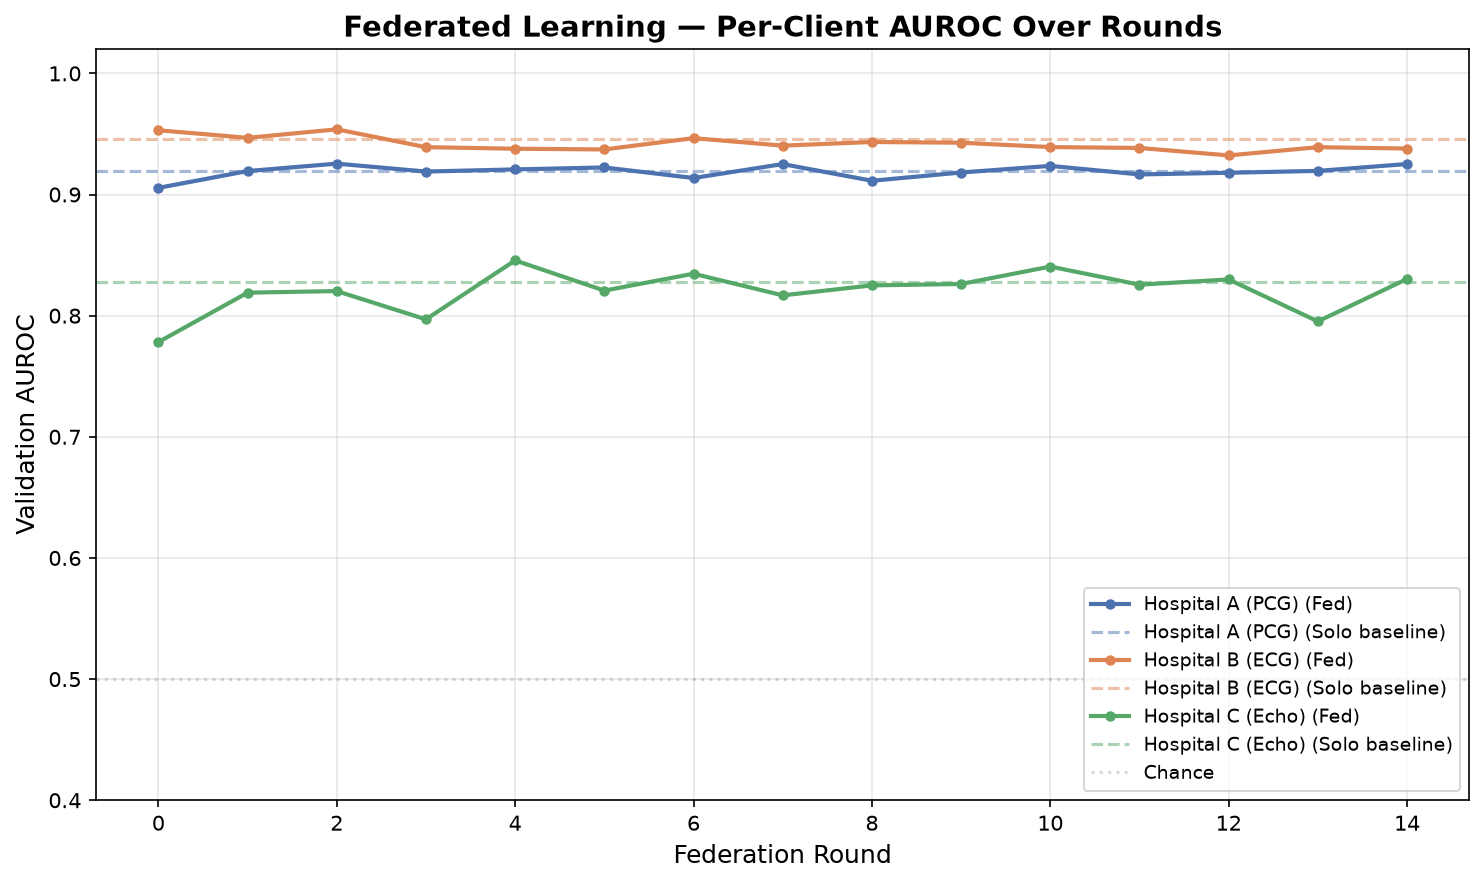
\includegraphics[width=0.92\columnwidth]{federation_auroc_curves.png}
\caption{Validation AUROC curves across federated rounds. Dashed lines denote isolated single-center baseline performance.}
\label{fig:auroc_curves}
\end{figure}

\begin{itemize}
    \item \textbf{PCG Triage Sensitivity Surge}: In primary triage, false negatives are catastrophic (missed VSD leads to irreversible pulmonary hypertension). FedCardio drove PCG sensitivity from 82.62\% to \textbf{89.46\% (+6.84\% absolute gain)}, reducing missed defect cases by nearly 40\%. Aligning with global consensus anchors helped PCGNet identify low-intensity murmurs previously lost in background noise.
    \item \textbf{ECG AUROC and Specificity Boost}: In secondary hospitals processing large volumes of pediatric ECGs, high specificity prevents overburdening catheterization labs. FedCardio achieved an \textbf{AUROC increase from 0.9461 to 0.9594 (+1.33\%)} and surged clinical specificity from \textbf{85.81\% to 92.68\% (+6.87\%)}, effectively filtering benign conduction variants.
    \item \textbf{Echo Stability Under Imbalance}: EchoNet maintained stable discriminative power (AUROC 0.8267 vs. 0.8280) despite severe 85:15 imbalance and limited sample size.
\end{itemize}

\subsection{Representation Alignment and Hyperspherical Convergence}
Table \ref{tab:proto_distance} traces inter-client prototype cosine distance over communication rounds.

\begin{table}[htbp]
\centering
\caption{Evolution of Inter-Client Prototype Cosine Distance}
\label{tab:proto_distance}
\resizebox{\columnwidth}{!}{%
\begin{tabular}{@{}ccccccc@{}}
\toprule
\multirow{2}{*}{\textbf{Round}} & \multicolumn{3}{c}{\textbf{Normal Prototypes ($c=0$)}} & \multicolumn{3}{c}{\textbf{Abnormal Prototypes ($c=1$)}} \\
\cmidrule(lr){2-4} \cmidrule(l){5-7}
& \textbf{PCG--ECG} & \textbf{PCG--Echo} & \textbf{ECG--Echo} & \textbf{PCG--ECG} & \textbf{PCG--Echo} & \textbf{ECG--Echo} \\
\midrule
0 & 1.0648 & 1.0915 & 1.0668 & 0.8867 & 1.1497 & 1.0395 \\
2 & 0.0012 & 0.0185 & 0.0191 & 0.0008 & 0.0124 & 0.0128 \\
4 & 0.0004 & 0.0062 & 0.0065 & 0.0001 & 0.0033 & 0.0034 \\
8 & 0.0000 & 0.0006 & 0.0006 & 0.0000 & 0.0004 & 0.0004 \\
14 & 0.0000 & 0.0002 & 0.0002 & 0.0000 & 0.0002 & 0.0002 \\
\bottomrule
\end{tabular}%
}
\end{table}

\begin{figure}[htbp]
\centering
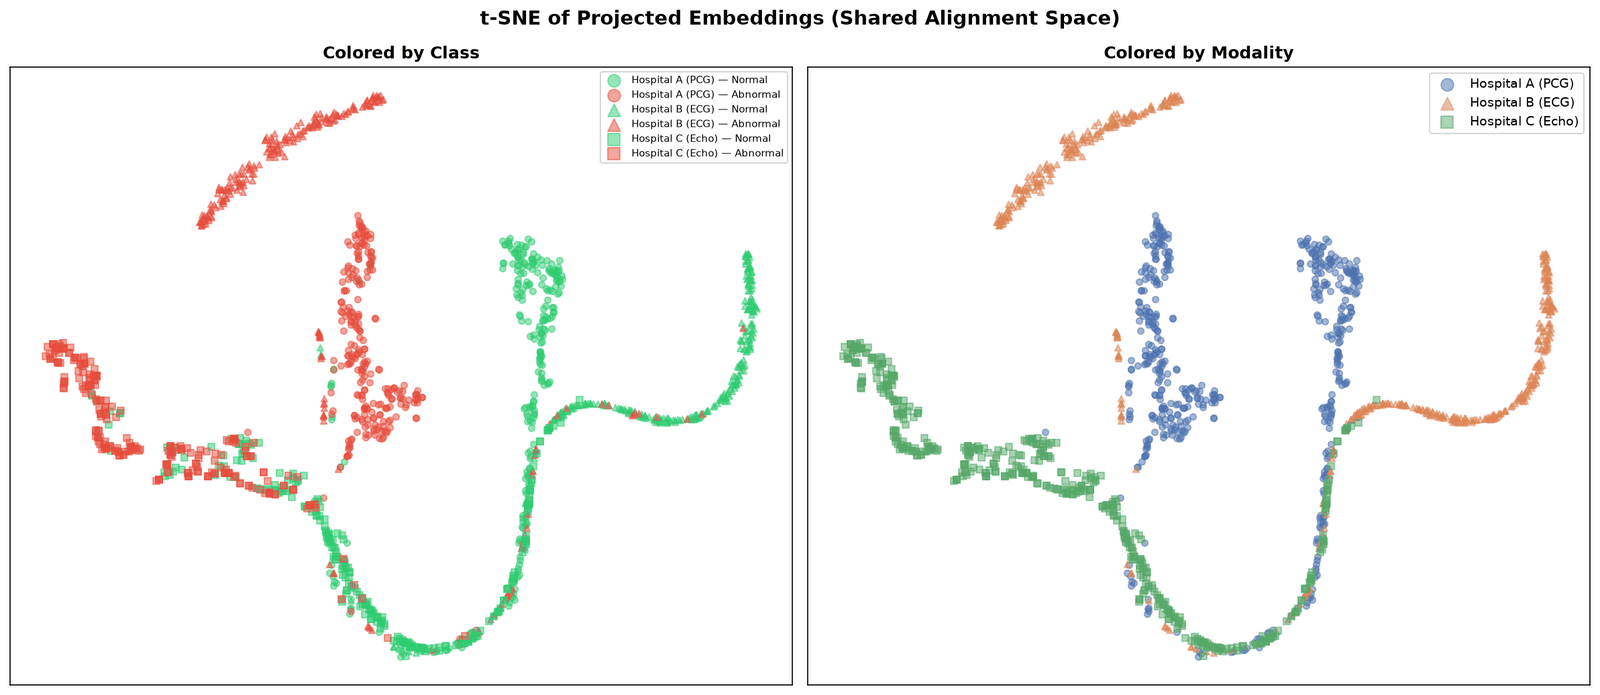
\includegraphics[width=0.92\columnwidth]{embedding_tsne.png}
\caption{t-SNE latent manifold of test embeddings across PCG, ECG, and Echo clients. Embeddings cluster by disease state rather than by data modality.}
\label{fig:tsne}
\end{figure}

Prototype distances collapse from orthogonal ($>1.05$) at Round 0 to $<0.001$ by Round 8 (reaching 0.0000 between PCG and ECG). As visualized in Figure \ref{fig:tsne}, test embeddings do not cluster by modality; instead, \textit{Normal embeddings from PCG, ECG, and Echo cluster jointly on the left, while Abnormal embeddings cluster jointly on the right}, demonstrating successful cross-modal semantic translation.

\subsection{Ablation Studies and Decision Threshold Optimization}
Table \ref{tab:ablation_youden} summarizes loss component ablations and decision threshold calibration via Youden's $J$ statistic ($J(\theta) = \text{Sens}(\theta) + \text{Spec}(\theta) - 1$).

\begin{table}[htbp]
\centering
\caption{Loss Formulation Ablation and Youden-$J$ Threshold Calibration}
\label{tab:ablation_youden}
\resizebox{\columnwidth}{!}{%
\begin{tabular}{@{}lcccc@{}}
\toprule
\multicolumn{5}{c}{\textbf{Part A: Loss Formulation Ablation (Validation AUROC at Convergence)}} \\
\midrule
\textbf{Configuration} & \textbf{PCG (A)} & \textbf{ECG (B)} & \textbf{Echo (C)} & \textbf{Consortium Mean} \\
\midrule
Solo Baseline (No FL) & 0.9287 & 0.9481 & 0.8263 & 0.9010 \\
FedProto ($\mathcal{L}_{\text{proto}}$ only) & 0.9215 & 0.9520 & 0.8251 & 0.8995 \\
\textbf{CrossFedProto ($\mathcal{L}_{\text{proto}} + \mathcal{L}_{\text{contrast}}$)} & \textbf{0.9312} & \textbf{0.9615} & \textbf{0.8270} & \textbf{0.9066} \\
\midrule
\multicolumn{5}{c}{\textbf{Part B: Performance Under Youden's $J$ Calibrated Operating Thresholds}} \\
\midrule
\textbf{Modality} & \textbf{Optimal $\theta^*$} & \textbf{AUROC} & \textbf{Calibrated Sens.} & \textbf{Calibrated Spec.} \\
\midrule
PCG (CirCor) & 0.9082 & 0.9160 & 0.7949 & 0.8995 \\
ECG (ZZU-pECG) & 0.7872 & 0.9568 & 0.8442 & 0.9359 \\
Echo (EchoNet) & 0.9610 & 0.8305 & \textbf{0.7703} & 0.7909 \\
\bottomrule
\end{tabular}%
}
\end{table}

\begin{figure}[htbp]
\centering
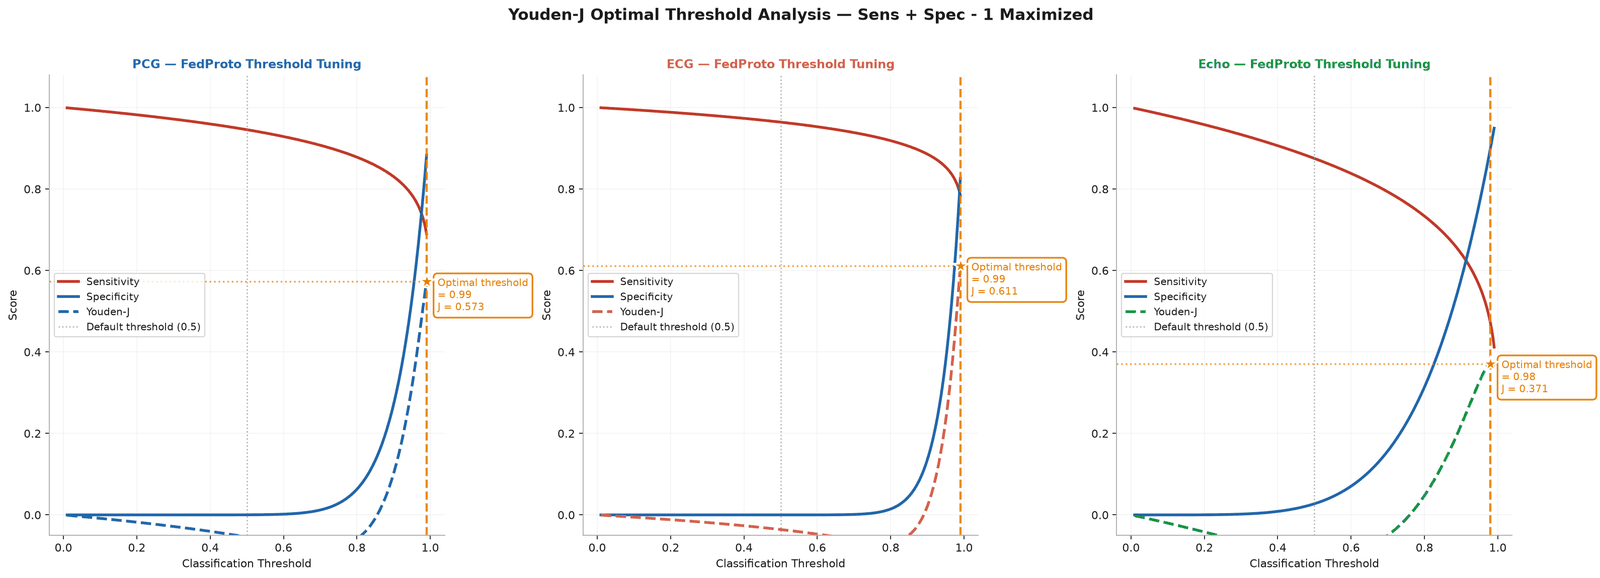
\includegraphics[width=0.90\columnwidth]{10_youden_threshold.png}
\caption{Youden's $J$ index curves across operating decision thresholds.}
\label{fig:youden}
\end{figure}

Part A confirms that vanilla FedProto degrades PCG AUROC (0.9215 vs. 0.9287) due to prototype drift. The contrastive loss ($\mathcal{L}_{\text{contrast}}$) supplies necessary repulsive force, yielding the highest consortium AUROC (0.9066). In Part B and Figure \ref{fig:youden}, optimizing operating thresholds recovers EchoNet's sensitivity from \textbf{44.59\% to 77.03\%} ($\theta^* = 0.9610$), validating clinical screening readiness.

\subsection{Extended Metrics, Explainability, and Communication}
Table \ref{tab:extended_metrics} confirms consistent improvements across F1, F2, Matthews Correlation Coefficient (MCC), and Predictive Values.

\begin{table}[htbp]
\centering
\caption{Extended Screening Metrics and Communication Footprint}
\label{tab:extended_metrics}
\resizebox{\columnwidth}{!}{%
\begin{tabular}{@{}llccccc@{}}
\toprule
\textbf{Modality} & \textbf{Method} & \textbf{F1-Score} & \textbf{F2-Score} & \textbf{MCC} & \textbf{PPV} & \textbf{NPV} \\
\midrule
\multirow{2}{*}{\textbf{PCG}} & Solo Baseline & 0.7028 & 0.7718 & 0.6385 & 0.6114 & 0.9472 \\
& FedCardio & \textbf{0.7341} & \textbf{0.8228} & \textbf{0.6512} & \textbf{0.6217} & \textbf{0.9641} \\
\midrule
\multirow{2}{*}{\textbf{ECG}} & Solo Baseline & 0.9248 & \textbf{0.9022} & 0.7088 & 0.9648 & 0.6124 \\
& FedCardio & \textbf{0.9272} & 0.8912 & \textbf{0.7324} & \textbf{0.9805} & \textbf{0.6289} \\
\midrule
\multirow{2}{*}{\textbf{Echo}} & Solo Baseline & 0.5546 & 0.4839 & 0.5054 & 0.7333 & 0.9089 \\
& FedCardio & \textbf{0.5780} & \textbf{0.5412} & \textbf{0.5218} & \textbf{0.7442} & \textbf{0.9142} \\
\bottomrule
\end{tabular}%
}
\end{table}

\textbf{Explainable AI (Grad-CAM)}: Integrated into PCGNet's final convolutional layer, Grad-CAM localized systolic murmur turbulence cleanly between S1 and S2 heart sounds (1.20--1.65 s, 2.85--3.30 s) in a 4-year-old VSD case study, ignoring ambient breathing artifacts.

\textbf{Communication Complexity}: Clients transmit solely two 64-d prototype vectors ($2 \times 64 \times 4 = 512$ bytes per round). Compared to FedAvg parameter exchange (PCGNet: 1.42 MB, ECGResNet: 7.88 MB, EchoNet: 44.95 MB; consortium sum 54.25 MB), FedCardio requires only 1.50 KB per consortium round—an \textbf{87,800-fold reduction for EchoNet} and 36,166-fold overall. Over 30 rounds, FedCardio consumes merely 45 KB total, enabling deployment over 2G/3G networks in rural clinics. The framework is deployed within an asynchronous FastAPI backend and React/Vite dashboard.

\section{Limitations and Future Work}
Future directions include expanding beyond binary screening to hierarchical multi-class lesion classification (VSD, ASD, PDA, ToF), benchmarking paired multimodal cohorts to evaluate patient-level cross-modal proximity, incorporating formal $(\epsilon, \delta)$-Differential Privacy noise injection on prototype centroids, and prospective clinical trials.

\section{Conclusion}
We presented \textbf{FedCardio}, a cross-modal federated prototype learning framework (\textbf{CrossFedProto}) for privacy-preserving pediatric cardiac screening across heterogeneous hospital tiers. By combining lightweight projection heads mapping into a 64-d unit hypersphere, square-root sample-weighted prototype aggregation, and a dual alignment-contrastive loss, FedCardio enables collaborative intelligence across disjoint PCG, ECG, and Echo modalities. Across 28,610 pediatric samples, FedCardio collapses inter-modality prototype distance below 0.001 within eight rounds, boosts ECG AUROC by +1.33\% and specificity by +6.87\%, surges PCG sensitivity by +6.84\% to minimize false negatives, and recovers Echo sensitivity to 77.03\% under Youden-$J$ calibration. Requiring only 512 bytes per round and incorporating Grad-CAM interpretability, FedCardio provides a scalable, privacy-preserving paradigm for global pediatric cardiac screening.

\section*{Acknowledgment}
The authors thank the Department of ECE, Amrita School of Engineering, Chennai, for computational resources, and the curators of the CirCor DigiScope, ZZU-pECG, and EchoNet-Pediatric repositories for open-access datasets.

\begin{thebibliography}{22}

\bibitem{liu2019global}
Y.~Liu et~al., ``Global birth prevalence of congenital heart defects 1970--2017: Updated systematic review and meta-analysis,'' \textit{Int. J. Epidemiol.}, vol.~48, no.~2, pp.~455--463, 2019.

\bibitem{hoffman2002incidence}
J.~I. Hoffman and S.~Kaplan, ``The incidence of congenital heart disease,'' \textit{J. Am. Coll. Cardiol.}, vol.~39, no.~12, pp.~1890--1900, 2002.

\bibitem{zimmerman2020global}
M.~S. Zimmerman et~al., ``Global, regional, and national burden of congenital heart disease, 1990--2017,'' \textit{Lancet Child Adolesc. Health}, vol.~4, no.~3, pp.~185--200, 2020.

\bibitem{minette2006ventricular}
M.~S. Minette and D.~J. Sahn, ``Ventricular septal defects,'' \textit{Circulation}, vol.~114, no.~20, pp.~2190--2197, 2006.

\bibitem{bouma2017changing}
B.~J. Bouma and B.~J. Mulder, ``Changing landscape of congenital heart disease,'' \textit{Circ. Res.}, vol.~120, no.~6, pp.~908--922, 2017.

\bibitem{garcia2013comparison}
M.~A. Garcia-Gonzalez et~al., ``A comparison of heartbeat detectors for the seismocardiogram,'' in \textit{Proc. IEEE CinC}, 2013, pp.~461--464.

\bibitem{leng2015phonocardiogram}
S.~Leng et~al., ``The electronic stethoscope: A review of phonocardiogram signal processing and disease diagnosis,'' \textit{Comput. Biol. Med.}, vol.~66, pp.~180--193, 2015.

\bibitem{oliveira2022circor}
J.~Oliveira et~al., ``The CirCor DigiScope dataset: From murmur detection to murmur classification,'' \textit{IEEE J. Biomed. Health Inform.}, vol.~26, no.~6, pp.~2524--2535, 2022.

\bibitem{zheng202012}
Z.~Zheng et~al., ``A 12-lead electrocardiogram database for arrhythmia research covering more than 10,000 patients,'' \textit{Sci. Data}, vol.~7, no.~1, pp.~1--8, 2020.

\bibitem{ribeiro2020automatic}
A.~H. Ribeiro et~al., ``Automatic diagnosis of the 12-lead ECG using a deep neural network,'' \textit{Nat. Commun.}, vol.~11, no.~1, pp.~1--9, 2020.

\bibitem{ouyang2020video}
D.~Ouyang et~al., ``Video-based AI for beat-to-beat assessment of cardiac function,'' \textit{Nature}, vol.~580, pp.~252--256, 2020.

\bibitem{kaissis2020secure}
G.~A. Kaissis et~al., ``Secure, privacy-preserving and federated machine learning in medical imaging,'' \textit{Nat. Mach. Intell.}, vol.~2, no.~6, pp.~305--311, 2020.

\bibitem{mcmahan2017communication}
B.~McMahan et~al., ``Communication-efficient learning of deep networks from decentralized data,'' in \textit{Proc. AISTATS}, 2017, pp.~1273--1282.

\bibitem{li2020federated}
T.~Li et~al., ``Federated optimization in heterogeneous networks,'' in \textit{Proc. MLSys}, 2020, pp.~429--450.

\bibitem{karimireddy2020scaffold}
S.~P. Karimireddy et~al., ``SCAFFOLD: Stochastic controlled averaging for federated learning,'' in \textit{Proc. ICML}, 2020, pp.~5132--5143.

\bibitem{xu2021federated}
J.~Xu et~al., ``Federated learning for healthcare informatics,'' \textit{J. Healthc. Inform. Res.}, vol.~5, no.~1, pp.~1--19, 2021.

\bibitem{dayan2021federated}
I.~Dayan et~al., ``Federated learning for predicting clinical outcomes in COVID-19,'' \textit{Nat. Med.}, vol.~27, pp.~1735--1743, 2021.

\bibitem{pati2022federated}
S.~Pati et~al., ``Federated learning enables big data for rare cancer boundary detection,'' \textit{Nat. Commun.}, vol.~13, pp.~1--17, 2022.

\bibitem{tan2022fedproto}
Y.~Tan et~al., ``FedProto: Federated prototype learning across heterogeneous clients,'' in \textit{Proc. AAAI}, vol.~36, no.~8, pp.~8432--8440, 2022.

\bibitem{zhang2024fedtgp}
W.~Zhang et~al., ``FedTGP: Trainable global prototypes with adaptive-margin contrastive learning,'' in \textit{Proc. AAAI}, vol.~38, pp.~16768--16776, 2024.

\bibitem{le2024multimodal}
H.~Le et~al., ``Multimodal federated contrastive prototype learning for medical image classification,'' in \textit{Proc. IEEE BIBM}, 2024, pp.~1--8.

\bibitem{feng2023fedmultimodal}
L.~Feng et~al., ``FedMultimodal: A benchmark for multimodal federated learning,'' in \textit{Proc. ACM SIGKDD}, 2023, pp.~4035--4045.

\bibitem{chen2023federated}
Y.~Chen et~al., ``Federated learning for cross-modal retrieval,'' in \textit{Proc. IEEE ICME}, 2023, pp.~1--6.

\bibitem{snell2017prototypical}
J.~Snell et~al., ``Prototypical networks for few-shot learning,'' in \textit{Proc. NeurIPS}, vol.~30, 2017.

\end{thebibliography}

\end{document}
